%% Figura standalone per la submission IEEE JBHI.
%% Compilare con: pdflatex fig2_rq2_governance.tex -> PDF vettoriale, font incorporati.
%% Font Times (ptm) per corrispondere a ieeecolor.cls.
%% Larghezza di destinazione: pagina piena (figure*, ~18.2 cm).
\documentclass[tikz,border=1pt]{standalone}
\renewcommand{\rmdefault}{ptm}
\usepackage{amsmath,amssymb}
\usetikzlibrary{positioning, arrows.meta, shapes.geometric}

%% Palette categoriale validata (slot 1 blu, slot 2 arancio).
\definecolor{serRaw}{HTML}{2A78D6}
\definecolor{serOPA}{HTML}{EB6834}
\definecolor{inkMuted}{HTML}{52514E}

\begin{document}
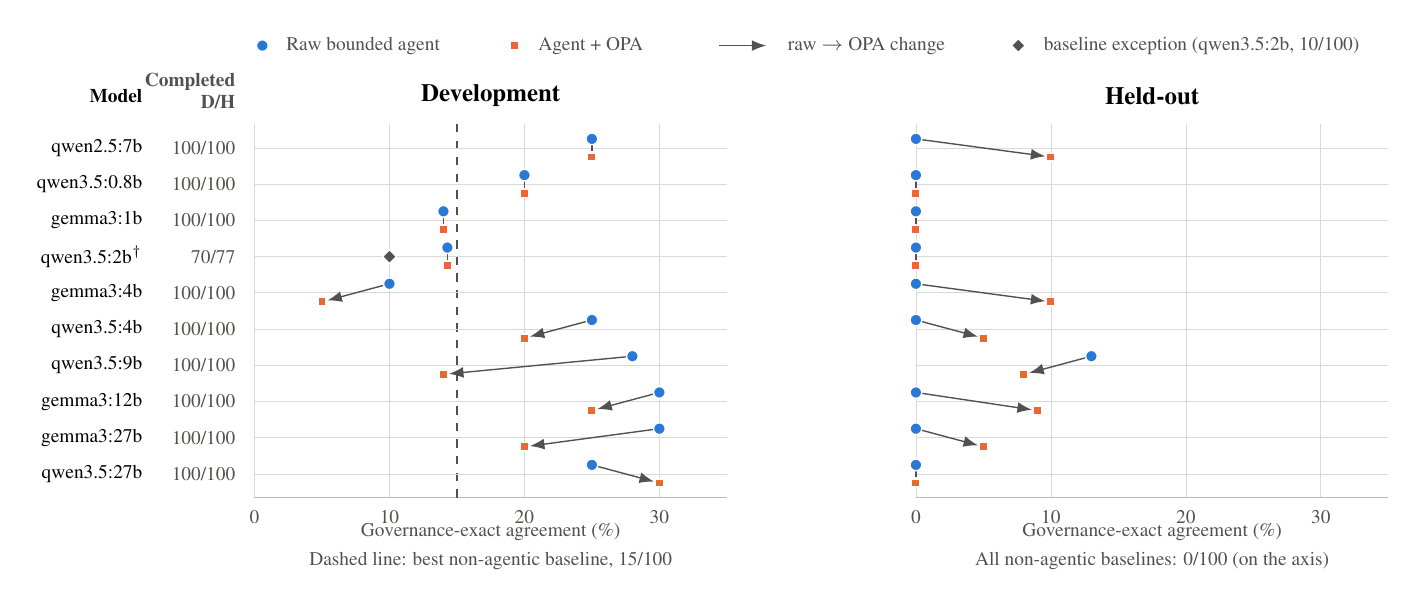
\begin{tikzpicture}[
  raw/.style={circle, fill=serRaw, draw=white, line width=0.5pt, inner sep=1.5pt},
  governed/.style={rectangle, fill=serOPA, draw=white, line width=0.5pt, inner sep=1.5pt},
  exception/.style={diamond, fill=inkMuted, draw=white, line width=0.5pt, inner sep=1.3pt},
  tick/.style={font=\scriptsize, text=inkMuted},
  model/.style={font=\scriptsize, anchor=east},
  compl/.style={font=\scriptsize, text=inkMuted, anchor=east},
  panel/.style={font=\small\bfseries},
  note/.style={font=\scriptsize, text=inkMuted},
  >=Latex
]
  %% --- geometria (unita': cm) ---
  \def\rowsep{0.46}          % passo verticale fra modelli
  \def\xs{0.1714}            % cm per punto percentuale (0--35 -> 6.0 cm)
  \def\pw{6.0}               % larghezza pannello
  \def\held{8.4}             % offset orizzontale del pannello held-out
  \def\dy{0.115}             % scostamento verticale fra marker sovrapposti
  \pgfmathsetmacro{\ytop}{9*\rowsep}

  %% --- griglia e assi dei due pannelli ---
  \foreach \off in {0,\held} {
    \foreach \v in {0,10,20,30} {
      \pgfmathsetmacro{\xx}{\off+\v*\xs}
      \draw[gray!30, line width=0.25pt] (\xx,-0.30) -- (\xx,{\ytop+0.30});
      \node[tick, below] at (\xx,-0.34) {\v};
    }
    \draw[gray!55, line width=0.4pt] (\off,-0.30) -- ({\off+\pw},-0.30);
  }

  %% --- linea di riferimento per il baseline non agentico (sviluppo) ---
  %% 15/100 per nove modelli su dieci: sostituisce dieci marker ridondanti.
  %% Nel pannello held-out il baseline vale 0/100 per tutti e dieci i modelli
  %% e coincide con l'asse, quindi non si traccia alcuna linea: si annota sotto.
  \draw[inkMuted, dashed, line width=0.6pt]
    ({15*\xs},-0.30) -- ({15*\xs},{\ytop+0.30});

  %% --- righe: modello, completamento, marker ---
  \foreach \name/\compD/\compH/\drawv/\dopa/\hraw/\hopa [count=\i from 0] in {
    qwen2.5:7b/100/100/25/25/0/10,
    qwen3.5:0.8b/100/100/20/20/0/0,
    gemma3:1b/100/100/14/14/0/0,
    qwen3.5:2b$^{\dagger}$/70/77/14.29/14.29/0/0,
    gemma3:4b/100/100/10/5/0/10,
    qwen3.5:4b/100/100/25/20/0/5,
    qwen3.5:9b/100/100/28/14/13/8,
    gemma3:12b/100/100/30/25/0/9,
    gemma3:27b/100/100/30/20/0/5,
    qwen3.5:27b/100/100/25/30/0/0
  } {
    \pgfmathsetmacro{\yy}{9*\rowsep-\i*\rowsep}
    \node[model] at (-1.30,\yy) {\name};
    \node[compl] at (-0.12,\yy) {\compD/\compH};
    \foreach \off in {0,\held} {
      \draw[gray!30, line width=0.3pt] (\off,\yy) -- ({\off+\pw},\yy);
    }

    %% sviluppo: raw -> +OPA. La punta di freccia compare solo se OPA
    %% sposta davvero il valore; altrimenti resterebbe una freccia verticale
    %% leggibile per errore come una diminuzione.
    \pgfmathsetmacro{\ddev}{abs(\dopa-\drawv)}
    \ifdim\ddev pt>0.01pt
      \draw[inkMuted, ->, line width=0.5pt, shorten <=2pt, shorten >=2pt]
        ({\drawv*\xs},{\yy+\dy}) -- ({\dopa*\xs},{\yy-\dy});
    \else
      \draw[inkMuted, line width=0.5pt, shorten <=2pt, shorten >=2pt]
        ({\drawv*\xs},{\yy+\dy}) -- ({\dopa*\xs},{\yy-\dy});
    \fi
    \node[raw]      at ({\drawv*\xs},{\yy+\dy}) {};
    \node[governed] at ({\dopa*\xs},{\yy-\dy}) {};

    %% held-out: raw -> +OPA
    \pgfmathsetmacro{\dhel}{abs(\hopa-\hraw)}
    \ifdim\dhel pt>0.01pt
      \draw[inkMuted, ->, line width=0.5pt, shorten <=2pt, shorten >=2pt]
        ({\held+\hraw*\xs},{\yy+\dy}) -- ({\held+\hopa*\xs},{\yy-\dy});
    \else
      \draw[inkMuted, line width=0.5pt, shorten <=2pt, shorten >=2pt]
        ({\held+\hraw*\xs},{\yy+\dy}) -- ({\held+\hopa*\xs},{\yy-\dy});
    \fi
    \node[raw]      at ({\held+\hraw*\xs},{\yy+\dy}) {};
    \node[governed] at ({\held+\hopa*\xs},{\yy-\dy}) {};
  }

  %% eccezione al baseline di sviluppo: qwen3.5:2b a 10/100 anziche' 15/100
  \pgfmathsetmacro{\yex}{9*\rowsep-3*\rowsep}
  \node[exception] at ({10*\xs},\yex) {};

  %% --- intestazioni di colonna e di pannello ---
  \node[model, font=\scriptsize\bfseries] at (-1.30,{\ytop+0.66}) {Model};
  \node[compl, font=\scriptsize\bfseries, align=right] at (-0.12,{\ytop+0.72}) {Completed\\D/H};
  \node[panel] at ({\pw/2},{\ytop+0.66}) {Development};
  \node[panel] at ({\held+\pw/2},{\ytop+0.66}) {Held-out};

  \node[tick] at ({\pw/2},-0.74) {Governance-exact agreement (\%)};
  \node[tick] at ({\held+\pw/2},-0.74) {Governance-exact agreement (\%)};

  %% --- annotazioni del baseline, sotto l'asse per non coprire i dati ---
  \node[note] at ({\pw/2},-1.10)
    {Dashed line: best non-agentic baseline, 15/100};
  \node[note] at ({\held+\pw/2},-1.10)
    {All non-agentic baselines: 0/100 (on the axis)};

  %% --- legenda ---
  \pgfmathsetmacro{\ylg}{\ytop+1.30}
  \node[raw] at (0.10,\ylg) {};
  \node[tick, anchor=west] at (0.28,\ylg) {Raw bounded agent};
  \node[governed] at (3.30,\ylg) {};
  \node[tick, anchor=west] at (3.48,\ylg) {Agent + OPA};
  \draw[inkMuted, ->, line width=0.5pt] (5.90,\ylg) -- (6.50,\ylg);
  \node[tick, anchor=west] at (6.65,\ylg) {raw $\rightarrow$ OPA change};
  \node[exception] at (9.70,\ylg) {};
  \node[tick, anchor=west] at (9.90,\ylg) {baseline exception (qwen3.5:2b, 10/100)};
\end{tikzpicture}
\end{document}
